\documentclass[11pt, english, fleqn, DIV=15, headinclude, BCOR=2cm]{scrreprt}

\usepackage[
    color,
    bibatend,
]{../../header}

\graphicspath{{./}{../Figures/}}

\usepackage{needspace}

\usepackage{mathtools}
\usepackage{listings}

\lstset{
    basicstyle=\small\ttfamily,
}

\hypersetup{
    pdftitle=
}

\newcommand\mot{\textsc{mot}}

\usepackage{longtable}
\usepackage{subcaption}

\usepackage[all]{nowidow}

\subject{Lab report}
\title{Magneto-optical trap}
\subtitle{Experiment A248 -- Universität Bonn}
\author{%
    Martin Ueding \\
    \small{\href{mailto:mu@martin-ueding.de}{mu@martin-ueding.de}}
    \and
    Lino Lemmer \\
    \small{\href{mailto:l2@uni-bonn.de}{l2@uni-bonn.de}}
}

\date{\daterange{2016-04-25}{2016-04-26}}

\publishers{Tutor: Daniel Babik}

\begin{document}

\maketitle

\begin{abstract}
    In this experiment we set up a magneto-optical trap to catch rubidium
    atoms. After that we investigate basic properties of the trap and its
    components.
\end{abstract}

\tableofcontents

\chapter*{Permission to upload}

I, Martin Ueding, would like to scan and upload this lab report with your
corrections to my website \href{http://martin-ueding.de}{martin-ueding.de}.
There, the original lab report as well as the reviewed one will be licensed
under the “\href{http://creativecommons.org/licenses/by-sa/4.0/}{Creative
Commons Attribution-ShareAlike 4.0 International License}”. Is that okay with
you?

Yes $\Box$ \hspace{2cm} No $\Box$

\chapter{Theory}

\section{Optical cooling}

\subsection{Radiation pressure}

Light, being mediated by massless gauge bosons, has a quadratic dispersion
relation $E = cp$ with momentum $p = \hbar k$ and wave number $k$. An atom
which absorbs a photon will obtain its energy and also its momentum. While in
stimulated emission the momentum of the emitted photon points in the same
direction as the stimulating atom's momentum, spontaneous emission is isotropic
which leads to a net acceleration. This effect causes the so called radiation pressure.

\subsection{Red detuning}

To cool atoms down one has to make sure that only those atoms that move
towards the laser beam feel this pressure. This can be done using the Doppler
effect: In the rest system of the atom, that flies towards the laser beam, the
photons of the laser are blue detuned, with $\nu'=\nu(1+v/c)$, where $v$ is
the velocity of the atom. To get those atoms on resonance again one has to
detune the laser to the red.

\subsection{Optical molasses}

The force of a laser with intensity $I$ and detuning $\delta =
\omega_\text{laser}-\omega_\text{res}$ on an atom can be expressed as
\[
    F_\text{radiation} = \frac{\hbar k\Gamma}2\cdot\frac{I/I_\text{S}}{\del{2\frac{\delta -
    kv}\Gamma}^2 + 1 + I/I_\text{S}}\, ,
\]
where $k$ denotes the wave vector of the photons, $\Gamma$ the decay rate of
the excited state and $I_\text{S}$ the saturation intensity. If we want to cool
the force at $v=0$ should be zero, which is clearly not the case. To solve this
one uses two counterpropagating laser beams with the same detuning. For small
velocities this gives a frictional force:
\[
    F_\text{count} = \frac{8\hbar k^2\delta}{\Gamma}
    \frac{I/I_\text{S}}{\del{\del{2\delta/\Gamma}^2 + 1 + I/I_\text{S}}^2}
    \cdot v \underset{\delta<0}{=} -\alpha\cdot v \, .
\]
Applying three orthogonal pairs of lasers gives an effective deacceleration of
atoms in every direction and with this a cooling. This setup is known as
\emph{optical molasses}. This cooling process is limited by heating due to
spontaneous emission. This leads to the so called \emph{Doppler limit}:
\[
    T_\text{Doppler} = \frac{\hbar \Gamma}{2k_\text{B}} \, .
\]

\section{Magneto-optical trap}

Since the forces in the optical molasses are independent of space, the atoms
 diffuse out of the cooling area. Due to collisions
those atoms get heated up again. We need an additional force that keeps the
atoms inside that area. One possibility is to use a \emph{magneto optical trap}
(\mot).

To simplify the working principle we consider a two level system with one
possible transition ($F=0 \to F=1$). Also we add a 1-dimensional linear
increasing magnetic field without loss of generality along the $z$ axis, which is zero at
$z=0$. Due to the Zeeman effect we get a space-dependent energy splitting of
the three possible $F=1$ configurations, which causes a lowering of the $m=1$
state's energy for $z<0$ and a lowering of the $m=-1$ level for $z>0$ (see
Figure~\ref{fig:mot-principle}).

Now we add two counterpropagating laser beams with detuning $\delta<0$. If now
the laser beam propagating in positive $z$ direction has a $\sigma^+$ helicity
and the counterpropagating beam has a $\sigma^-$ helicity, atoms which are
located at $z<0$ have a higher possibility to absorb $\sigma^+$ photons and
hence get pushed back to $z=0$. For atoms at $z>0$ it is the other way around.
There the absorption of a $\sigma^-$ photon is more likely, so that they 
also get pushed back to $z=0$.

While in reality the energy levels are way more complex the working principle
remains the same.

\begin{figure}
    \centering
    \includegraphics{mot-principle}
    \caption{%
        Energy levels and transitions in a spatially varying magnetic field.
    }
    \label{fig:mot-principle}
\end{figure}

\section{Rubidium}

Natural rubidium consists about \SI{72}{\percent} of ${}^{85}\text{Ru}$ and
\SI{28}{\percent} of ${}^{87}\text{Ru}$. In our \mot{} we use the former.
Part of its hyperfine level scheme is shown in Figure~\ref{fig:rubidium85}. To
create a quasi two level system we use the closed $F=3 \to F'=4$ transition.
Since this is not a real two level system there is a finite probability for the
transition from $F'=4$ to $F=2$. In this state the atom can not be excited by
the cooling laser again. Therefor it is called \emph{dark state}. To solve this
problem a second laser, the \emph{pumping laser} excites the atoms in the dark
state to the $F'=3$ state, from where it can decay into the cooling ground
state $F=3$ again and with this get the atom back in the cooling cycle.

\begin{figure}
    \centering
    \includegraphics{rubidium85}
    \caption{%
        Part of the ${}^{85}\text{Ru}$ level scheme. The colored transitions
        are the ones used in this experiment. The cooling beam uses the red
        transition while the blue transition is needed for the repumping.
    }
    \label{fig:rubidium85}
\end{figure}

\section{Diode lasers}

A diode laser is a semiconductor diode, which works quite similar to a
\textsc{led}. Photons are produced in a highly doped p-n-junction by
recombination of electrons and holes. Due to partial reflection at the border
between diode material and the surrounding air the diode becomes a resonator,
which works as laser if more atoms are excited rather than in their ground
state. This can be reached by electrical pumping with a current in forward
direction of the diode. The frequency of the laser depends on the size of the
band gap.  Because of the large active region this so called \emph{homojunction
laser diode} is very ineffective as it needs a high current density.

For our case the better diode is a so called \emph{double-heterojunction laser
diode}, which consists of a thin layer of low band gap material, sandwiched
between two high band gap layers. This type requires a lower current
density, which allows continuous wave operation at room temperature. 

The frequency range of laser diodes is typically quite large. To get a narrow
line width and to stabilize the frequency one uses an external resonator. For
this the (divergent) laser beam gets focused on a diffraction grating. For all
wavelengths the reflected beam of 0th order points in the same direction, but
the angle of all other orders are frequency dependent. One chooses the position
of the grating so that the -1st order of the wanted frequency is coupled back
into the laser, which causes a strong amplification of that frequency. 

In this experiment the position of the grating can be controlled with a Piezo
element. This allows us to choose the frequency by the voltage on the Piezo.
One can now scan trough frequencies by applying a triangular voltage.

The diode laser setup is still sensitive to mechanical distortions. For a
further frequency stabilization an error signal is fed back to the Piezo.

\section{Doppler-free spectroscopy}

Since the Doppler broadening of spectral lines at room temperature is orders of
magnitude bigger than the natural line width, lines which lie close together can
not be resolved. To nevertheless investigate those lines one has to use
Doppler-free spectroscopy.

For this two counterpropagating laser beams of same frequency are needed, a
\emph{pump beam} and a \emph{probe beam} with lower intensity. The absorption
of the probe beam gets recorded. For a simple understanding again consider a
two level system with ground state $\ket{g}$, excited state $\ket{e}$ and
energy difference of $\hbar\omega_0$. If the lasers both have the frequency
$\omega_0$ atoms with $v\neq0$ along the laser's direction will be out of
resonance due to the Doppler effect. Those atoms with $v\approx 0$ will be
excited by the pump beam and hence the absorption of the probe beam is very
low. If the lasers are detuned to the red from the resonance frequency the pump
beam and the probe beam excite oncoming atoms with respect to their own
propagation direction. Therefor the absorption of the probe beam is high.
The same holds for blue detuned lasers. This leads to a transmission spectrum as
in Figure~\ref{fig:doppler-free-2-level}. If one takes an absorption
spectrum one gets dips instead of peaks, which are called \emph{Lamb dips}.

In reality there will be more levels, which makes the absorption spectrum more
complex. Take for example a system with one ground level and two excited level
with excitation energy $\hbar\omega_1$ and $\hbar\omega_2$ respectively. When
we apply the same method as above it can happen, that the pump beam is on
resonance with one of the excited levels and the probe beam with the other.
This leads to a so called \emph{cross over peak} at $\omega_\text{probe} =
\frac{\omega_1+\omega_2}2$ (see Figure~\ref{fig:doppler-free-3-level}).

\begin{figure}
    \begin{subfigure}{.5\textwidth}
        \centering
        \includegraphics{doppler-free-2-level}
        \caption{%
            Two level system.
        }
        \label{fig:doppler-free-2-level}
    \end{subfigure}
    \hfill
    \begin{subfigure}{.5\textwidth}
        \centering
        \includegraphics{doppler-free-3-level}
        \caption{%
            Three level system.
        }
        \label{fig:doppler-free-3-level}
    \end{subfigure}
    \caption{%
        Transmission spectra in Doppler-free spectroscopy.
    }
\end{figure}

\section{Polarization spectroscopy}

The error signal for frequency stabilization can be obtained using polarization
spectroscopy. As the name implies this kind of spectroscopy uses the probe
beam's polarization rather than its intensity. The reason for this is, that one
can detect small changes in polarization much better than small changes in
intensity.

Polarization spectroscopy uses a setup similar to the one of the Doppler free
saturation spectroscopy. In contrast to the latter the pump beam is circular
polarized. Additionally there are two linear polarizers, one at each
end of the spectroscopy cell, which are crossed, so that the background
signal is suppressed.

Due to the circular polarized pumping beam ($\Deltaup m = \pm1$) the degenerate
$m$ states of the transition's excited level get unequally occupied, which
leads to an alignment different from the thermal equilibrium. The resulting
anisotropy shifts the polarization axis of the linear probe beam, which hence
can be detected. The precision is due to the crossed polarizers up to three
orders of magnitude better than the precision of the saturation spectroscopy.
If there is a small angle between the two beams and if the birefringence of the
cell's windows is reduced one can obtain a signal with a dispersive profile
which allows to detect small deviations of the wanted frequency. These can be
used to correct the grating's angle so that the frequency lock remains stable.

\chapter{Conduction}

\section{Apparatus}

Our setup consists of two blocks: the laser setup and the \mot\ setup. In the
laser setup (see Figure~\ref{fig:setup-laser}, we have two tunable lasers as
described in the chapter about theory. One will serve as a pumping laser, the
other one will be the cooling one. Both lasers are optically isolated using a
Faraday isolator. This relieves us from making sure that no light feeds back
into the laser system. Without the isolator, we would create a second laser
cavity which we do not want.

\begin{figure}
    \centering
    \begin{subfigure}[c]{0.47\linewidth}
        \centering
        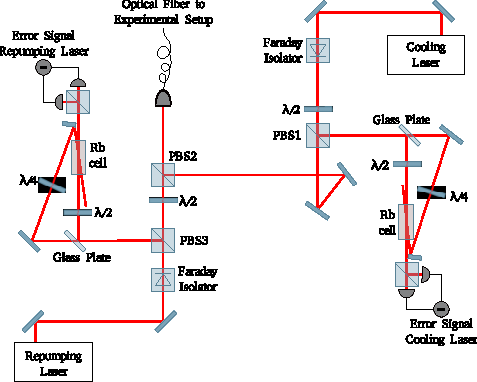
\includegraphics[width=\linewidth]{setup-laser}
        \caption{%
            Laser part
        }
        \label{fig:setup-laser}
    \end{subfigure}
    \hfill
    \begin{subfigure}[c]{0.47\linewidth}
        \centering
        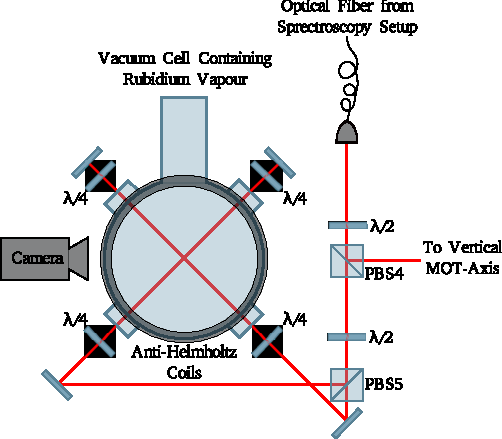
\includegraphics[width=\linewidth]{setup-mot}
        \caption{%
            \textsc{Mot} part
        }
        \label{fig:setup-mot}
    \end{subfigure}
    \caption{%
        Setup of the experiment. Both images are taken from the supplementary
        material.
    }
    \label{fig:setup}
\end{figure}

Each laser has an independent locking mechanism via polarization spectroscopy.
Part of the laser beam is taken away with a polarizing beam splitter and
analysed in a rubidium cell. The error signal from each laser is fed into a
lock box (not shown) to lock the laser into the desired frequency.

The light of the two lasers is combined into an optical fiber which leads the
light to the \mot\ setup shown in Figure~\ref{fig:setup-mot}. There we split
the light into three approximately equally powered beams using $\lambda/2$
plates and polarizing beam splitters. Each of the those three linearly
polarized beams is sent through a $\lambda/4$ plate to become circularly
polarized. That is then led through the \mot\ chamber and back again with
reversed polarization.

An annotated photo of the \mot\ setup is shown in
Figure~\ref{fig:setup_photo_annotated}. The colors of the beams are just to
help the eye, the beam itself always had the same IR \enquote{color}. The
individual elements are the following.

\begin{figure}
    \centering
    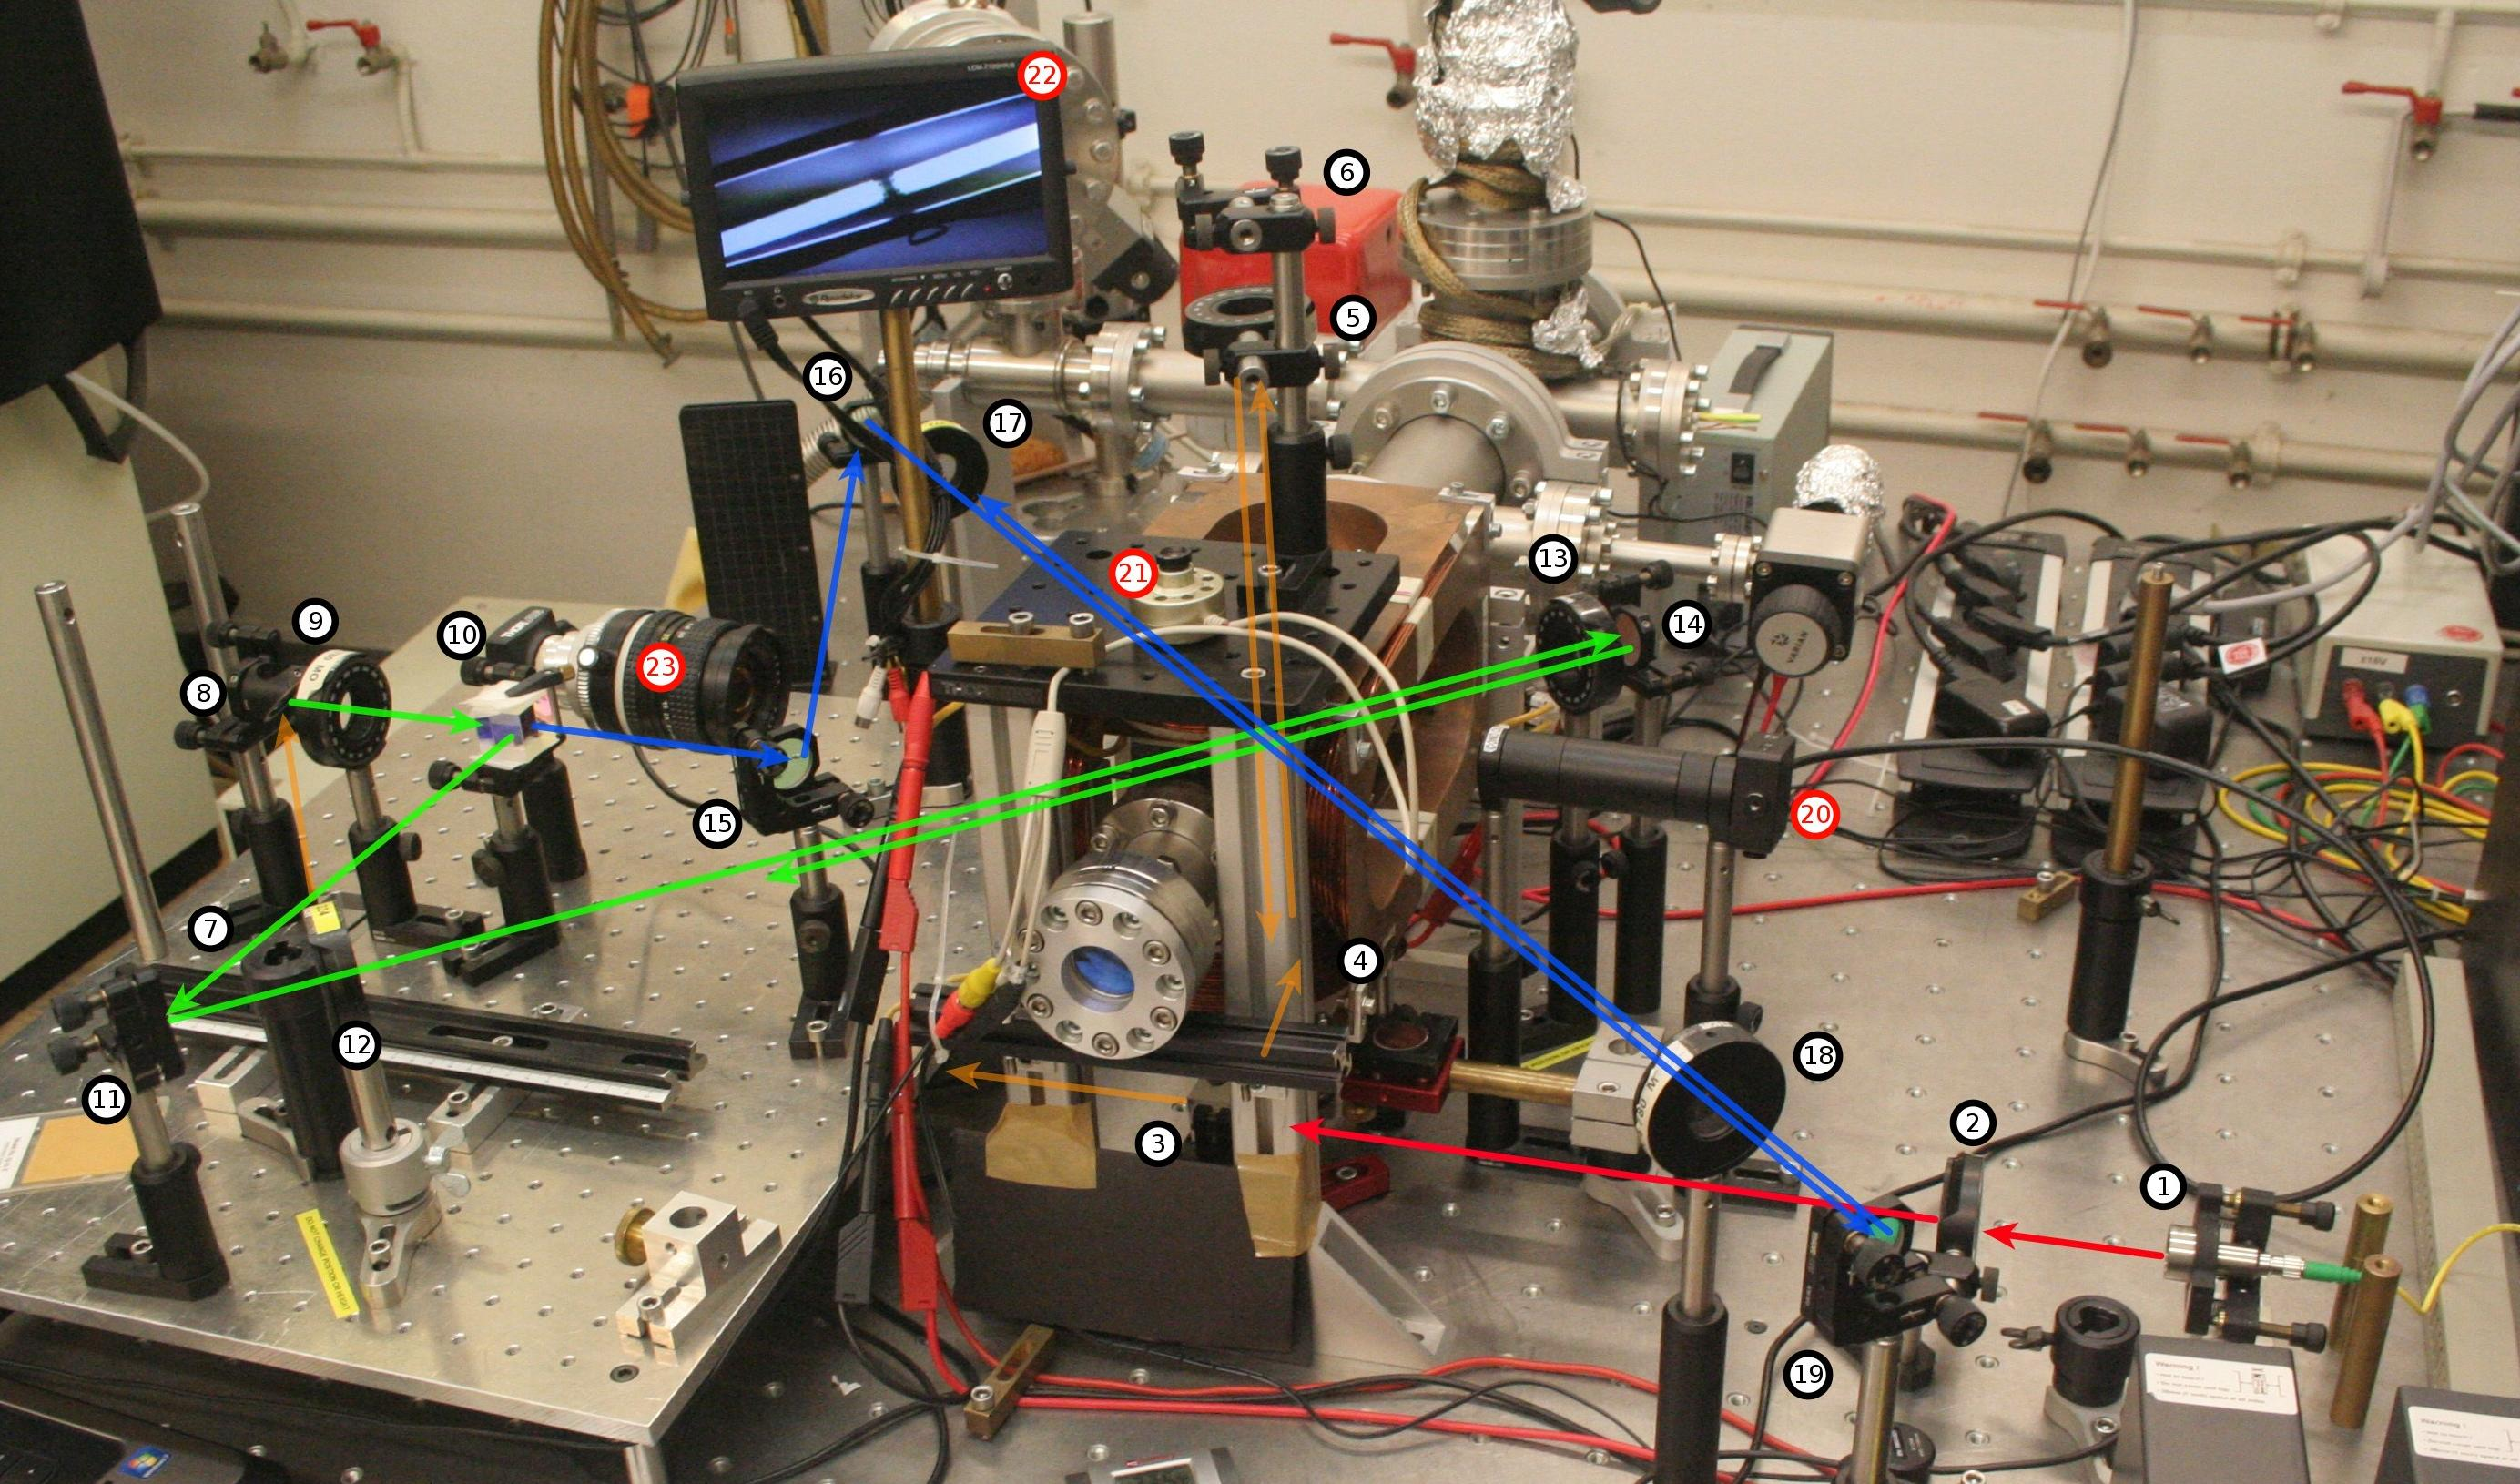
\includegraphics[width=\linewidth]{setup_photo_annotated}
    \caption{%
        Setup of the \mot. The arrows show the path of the light rays. Ray
        colors are for illustration only. Numbers are explained in the text.
    }
    \label{fig:setup_photo_annotated}
\end{figure}

\begin{enumerate}
    \item
        Exit of optical fiber. The combined light of cooling and pumping
        laser enters the \mot\ part of the experiment here.
    \item
        $\lambda/2$ plate. Adjusts the polarization of the light onto the beam
        splitter.
    \item
        Polarizing beam splitter. Splits the linearly polarized light in order
        to use one beam in the $z$-direction and the remainder in the
        transversal direction. By adjusting the $\lambda/2$ plate \textcircled
        2 in front, one can adjust the beam power splitting.
    \item
        Mirror and $\lambda/4$ plate. Reflects the incoming light upwards
        through the \mot\ chamber. The plate then makes the light circularly
        polarized.
    \item
        $\lambda/4$ plate.
    \item
        Mirror. Reflects the light back down.
    \item
        Mirror. Reflects one beam from \textcircled 3 upwards.
    \item
        Mirror. Directs the light back into the horizontal. \textcircled 7 and
        \textcircled 8 will be called \enquote{elevator} occasionally.
    \item
        $\lambda/2$ plate. Allows to adjust the splitting ratio with
        \textcircled{10}.
    \item
        Polarizing beam splitter. Splits the incoming beam into $x$ (blue) and
        $y$ (green) part.
    \item
        Mirror. Directs the $y$ beam into the \mot\ chamber.
    \item
        $\lambda/4$ plate. Makes the light (close to) circularly polarized.
    \item
        $\lambda/4$ plate.
    \item
        Mirror. Reflects the $y$ beam back through the chamber.
    \item
        Mirror. Moves the $x$ beam around the camera.
    \item
        Mirror. Directs the $x$ beam into the chamber.
    \item
        $\lambda/4$ plate. Same as \textcircled{12}.
    \item
        $\lambda/4$ plate. Same as \textcircled{13}.
    \item
        Mirror. Same as \textcircled{14}.
    \item
        Mount for photo diode or power meter.
    \item
        IR camera. Useful for setting up the lasers.
    \item
        Live screen for IR camera.
    \item
        Camera directed onto \mot. Needed for \mot\ size estimation.
\end{enumerate}

All the nine mirrors and three $\lambda/2$ have to be adjusted by us. The
six $\lambda/4$ plates are set to a decent setting from the start.

\section{Setup and calibration}

First we have to lock the cooling laser to the right transition. For this we
tune the laser roughly to the wanted frequency. The lock box gets a triangular
signal from a function generator, changes its amplitude and offset and gives it
to the piezo which controls the grating's position. The Doppler-free spectrum of
the $F=3$ ground state of ${}^{85}\text{Ru}$ is shown in
Figure~\ref{fig:doppler-free-cooling}. From there we choose the right line,
zoom in and lock the laser to a frequency a bit below the chosen transition. 

\begin{figure}
    \centering
    \includegraphics{doppler-free-cooling}
    \caption{%
        Doppler-free spectrum of the ${}^{85}\text{Ru}$ $F=3 \to F'=2,3,4$
        lines. The time is related to the lasing frequency via the triangular
        voltage applied to the piezo.
    }
    \label{fig:doppler-free-cooling}
\end{figure}

For the pumping laser we repeat the last steps. The Doppler-free spectrum of the
$F=2$ ground state of ${}^{85}\text{Ru}$ is shown in
Figure~\ref{fig:doppler-free-pumping}. The lines are so close together, that we
can not distinguish between them. Instead of trying to lock we quasi-lock by
zooming in far to the spot where we expect the right transition to be.

\begin{figure}
    \centering
    \includegraphics{doppler-free-pumping}
    \caption{%
        Doppler-free spectrum of the ${}^{85}\text{Ru}$ $F=2 \to F'=1,2,3$
        lines. The time is related to the lasing frequency via the triangular
        voltage applied to the piezo. Since one can not distinguish between
        lines, the labels are only rough estimates. 
    }
    \label{fig:doppler-free-pumping}
\end{figure}

Now we check if enough light is passing through the fiber. With the
powermeter we measure a total power of \SI{16.8}{\milli\watt}. Then be block
the path of the pumping laser and measure again. Now we get
\SI{14.1}{\milli\watt}. The instruction states the cooling laser needs to be at
least \SI{5}{\milli\watt} and the pumping laser \SI{1}{\milli\watt}, which both
is clearly the case for our setup.

After that we have to adjust the polarizing beam splitter and the mirrors. For
that we first check, if the first \textsc{pbs} and the bottom elevator mirrors
are hit nicely by the beam. As this is the case we modify the bottom
$z$-mirror's orientation such that the beam passes through the center of the
vacuum chamber. Then we adjust the top mirror such that the beams overlap
perfectly. This can be checked with the help of a camera, which is still
sensitive to the beam's wavelength.

Before we adjust the transversal ($x$ and $y$) beams we try to get equal light
power to each axis. So we measure the fiber power again, which is
\SI{15.1}{\milli\watt} and set the $z$-axis power to to \SI{5.0}{\milli\watt}
by rotating the $\lambda/2$ plate behind the fiber. Against our expectations we
then have no power on the transversal elevator. We try it the other way around
and adjust the $\lambda/2$ plate again until we have \SI{8.8}{\milli\watt} on
the elevator and \SI{4.8}{\milli\watt} on the $z$-axis.

After measuring the beam power directly in front of the vacuum chamber we
realize that we incur loss on all the mirrors and first adjust the splitting in
the transversal directions to be symmetric. There now are \SI{2.7}{\milli\watt}
on each of them. Then we adjust the initial $\lambda/2$ plate to give more
power to the transversal and less to the longitudinal direction. After that we
have \SI{3.1}{\milli\watt} behind each polarizing beam splitter.

We start to adjust the transversal mirrors. We calibrate the $y$ direction
first. When the reflected beam coincides nicely with the incident beam we move
on to the $x$ direction and repeat the procedure. 

After checking the locking of the lasers we tweak again on all the mirrors to
optimize the overlap. Now when toggling the power supply of the magnetic field,
we can see a little difference in the brightness which indicates a working
\mot. With the help of a photo diode we then adjust the laser locks to
make the \mot{} even larger.

\begin{table}
    \centering
    \begin{tabular}{SSS}
        \toprule
        {total power/\si{\nano\watt}}
        & {background/\si{\nano\watt}}
        & {power of \mot/\si{\nano\watt}} \\
        \midrule
        %< for row in power_mot_table >%
        << ' & '.join(row) >> \\
        %< endfor >%
        \bottomrule
    \end{tabular}
    \caption{%
        Measured powers. The third column is just the difference of the first
        two columns.
    }
    \label{tab:mot_power}
\end{table}

\section{MOT characterization}

\subsection{MOT population}

% TODO Make this a better heading.

The first attribute of our \mot{} is the number of caught atoms. For this we
have to find the fluorescence power. After replacing the photo diode with the
power meter, we see that out \mot{} is very bright, but not very constant in
power.  Therefor we measure a few times to find a mean value (see
Table~\ref{tab:mot_power}). Our \mot's power is hence \SI{<< power_mot
>>}{\nano\watt} which is quite good, as the instruction states that about
\SI{50}{\nano\watt} are needed. We also need the diameter of the lens and its
distance to the \mot. Since the lens is an \SI{1}{\inch} lens, its diameter is
\SI{2.54}{\centi\meter}. Its distance to the \mot{} is \SI{10}{\centi\meter},
roughly estimated. Then we need the beam's power. We measure on each axis
separately and get $P_x = \SI{3.57}{\milli\watt}$, $P_y =
\SI{3.36}{\milli\watt}$ and $P_z = \SI{4.45}{\milli\watt}$.

Another quantity we have to know is the beam diameter. For this we put a razor
blade on an optical rail in the $y$-beam and measure the remaining power
depending on the razor's position. Our measurements are shown in
Table~\ref{tab:beam_diameter}. At last we need the detuning of the cooling
laser. This will be estimated later on.

\begin{table}
    \centering
    \begin{tabular}{SS}
        \toprule
        {absolute position/\si{\centi\meter}}
        & {power of beam/\si{\milli\watt}} \\
        \midrule
        %< for row in beam_diameter_table >%
        << ' & '.join(row) >> \\
        %< endfor >%
        \bottomrule
    \end{tabular}
    \caption{%
        Measurement to estimate the beam diameter.
    }
    \label{tab:beam_diameter}
\end{table}

The collected data is also shown in Figure~\ref{fig:diameter} with a Gaussian
CDF fit. From the fit we derive a total beam power of \SI{<< beam_power
>>}{\milli\watt} and an $\eup^{-2}$ beam diameter of \SI{<< beam_diameter
>>}{\centi\meter}. Errors are estimated by the diagonal of the fit covariance
matrix.

\begin{figure}
    \centering
    \includegraphics{diameter}
    \caption{%
        Beam diameter measurement. Shown is the beam power that is left after
        moving the razor blade to the given position.
    }
    \label{fig:diameter}
\end{figure}


\subsection{Size of MOT}

Now we want an estimate of our \mot's size. For this we first take a picture of
the chamber with the \mot\ and without it. Then we subtract those images in
order to remove the background from the other laser beams. This is shown in
Figure~\ref{fig:difference-3-inv}.

Then we turn the camera and take a picture of a scale at the same distance. The
image of the centimeter scale is shown in Figure~\ref{fig:scale}. For a rough
estimation, the superposition of the \mot\ signal and the scale shown in
Figure~\ref{fig:motsize} can used. The radius of the \mot\ should be in the
neighborhood of say \SI{2}{\milli\meter}.

\begin{figure}
    \centering
    \includegraphics[width=.7\linewidth]{difference-3-inv.png}
    \caption{Substraction image showing the \mot.}
    \label{fig:difference-3-inv}
\end{figure}

\begin{figure}
    \begin{subfigure}{.45\textwidth}
        \centering
        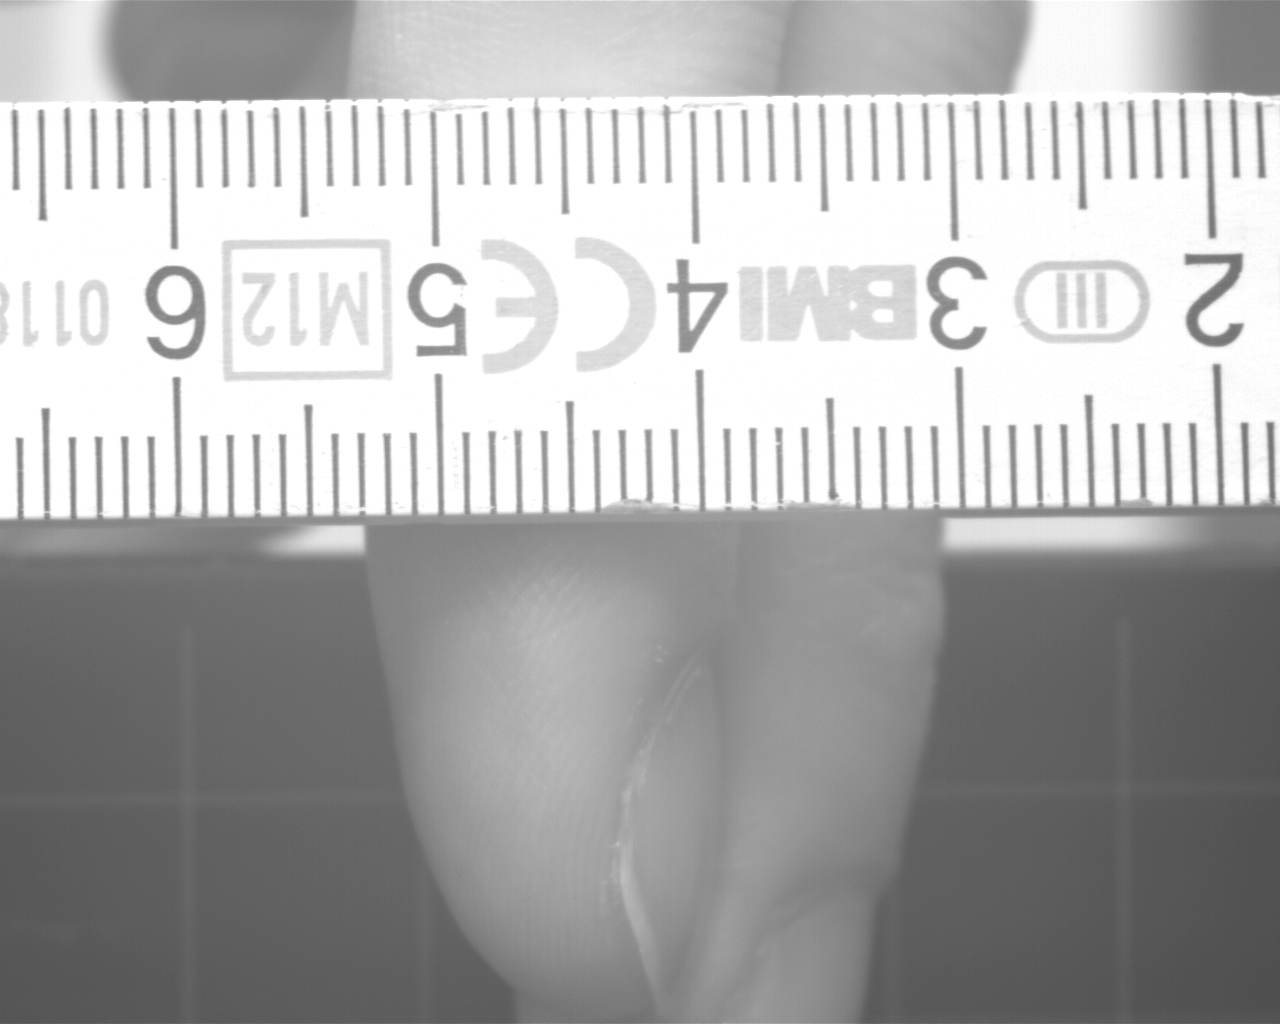
\includegraphics[width=\linewidth]{scale.png}
        \caption{Whole image of scale.}
        \label{fig:scale}
    \end{subfigure}
    \hfill
    \begin{subfigure}{.45\textwidth}
        \centering
        \includegraphics[width=\linewidth]{motsize}
        \caption{Superposition of \mot\ and scale.}
        \label{fig:motsize}
    \end{subfigure}
    \caption{Millimeter scale at the same distance as the \mot.}
    \label{fig:mot_size}
\end{figure}

We want to have a more exact estimation of this area. We therefore let the
computer sum the pixel values of a cropped version shown in
Figure~\ref{fig:mot-crop}. Then we divide by the difference in maximum and
minimum value. This should give an good estimation of the \mot\ size.

Our algorithm counts \num{<< mot_white_pixels >>} white pixels. Some dark gray
pixels contribute a bit, some light gray pixels do not contribute fully. We
hope that on average this works out. For comparison, the image used has \num{<<
mot_total_pixels >>} pixels.

We carefully choose two points on the millimeter scale which are
\SI{10}{\milli\meter} apart and near the spot where the \mot\ is on our images.
This reduces the statistical error a bit while not becoming too sensitive to
lens distortions. We conclude that in the focal plane of the camera, we can
convert with the constant \SI{<< mot_mm_per_pixel >>}{\milli\meter\per\pixel}
to physical sizes.\footnote{\si{\pixel} is the unit for pixels, at least in CSS
(Cascading Style Sheets).} From the number of white pixels, \num{<<
mot_white_pixels >>}, we conclude that we have a radius of \SI{<< mot_radius_px
>>}{\pixel} and thus \SI{<< mot_radius_mm >>}{\milli\meter} assuming that a
circle is a good approximation. Judging by Figure~\ref{fig:motsize}, this is a
sensible result. Converting this radius to a volume, we obtain a spherical
\mot\ volume of \SI{<< mot_volume_mm3 >>}{\milli\meter\cubed}.


\begin{figure}
    \centering
    \includegraphics[width=.3\linewidth]{mot-crop}
    \caption{%
        Selection used for area determination.
    }
    \label{fig:mot-crop}
\end{figure}

\subsection{Influence of quarter waveplates}

The effect of the $\lambda/4$ plates in front of the \mot{} is significant.
This is shown in Figure~\ref{fig:lambda_front}. Depending on the orientation of
the plates the beam behind the plate stays linearly or becomes elliptically or
circularly polarized. This can suppress the formation of the trap completely.
The effect of the plates in the backreflected beam can be seen in
Figure~\ref{fig:lambda_behind}. It is not very large. Ideally there should be
no change of the \mot's power, of course. The effect that we do see indicates
that the light is not perfectly circularly polarized.

\begin{figure}
    \centering
    \begin{subfigure}[c]{0.48\linewidth}
    \centering
    \includegraphics{lambda_front}
    \caption{%
        In front
    }
    \label{fig:lambda_front}
    \end{subfigure}
    \hfill
    \begin{subfigure}[c]{0.48\linewidth}
    \centering
    \includegraphics{lambda_behind}
    \caption{%
        Behind
    }
    \label{fig:lambda_behind}
    \end{subfigure}
    \caption{%
        Effect of the $\lambda/4$ plates around the vacuum chamber.
        % TODO What is the fit?
    }
    \label{fig:}
\end{figure}

\subsection{Influence of magnetic field}

Go through the magnetic field current.

% TODO Table with magnetic field.

% TODO Flesh out the paragraphs here.

The dependence of the \mot\ intensity on the external magnetic field current is
shown in Figure~\ref{fig:magnetic}.

\begin{figure}
    \centering
    \includegraphics{magnetic}
    \caption{%
        \mot\ response to a changing magnetic field. The points in the middle
        have been measured twice after we noticed some hysteresis effect.
    }
    \label{fig:magnetic}
\end{figure}

\subsection{Loading behavior}

Pressure is supposed to be \SIrange{1.1e-7}{1.5e-7}{\milli\bar}

Room temperature \SI{24}{\celsius}

To model the loading of the trap, we use a rising exponential with steady-state
load $N_0$, start time $t_0$ and the \enquote{lifetime} in the filling process,
\[
    N(t) = N_0 \sbr{1 - \exp\del{- \frac{t - t_0}{\tau}}} \,.
\]
% TODO Cite Wieman (1) here.

Figure~\ref{fig:loading} shows four of six measurements that we did for the
loading of the \mot. We have rescaled and shifted all signals from the
photodiode such that one can easily compare the signals visually.

\begin{figure}
    \centering
    \begin{subfigure}[c]{0.48\linewidth}
        \centering
        \includegraphics{loading-1}
        \caption{%
            %
            }
        \label{fig:/1}
    \end{subfigure}
    \hfill
    \begin{subfigure}[c]{0.48\linewidth}
        \centering
        \includegraphics[width=\linewidth]{loading-2}
        \caption{%
            %
            }
        \label{fig:/2}
    \end{subfigure}

    \begin{subfigure}[c]{0.48\linewidth}
        \centering
        \includegraphics{loading-3}
        \caption{%
            %
            }
        \label{fig:/1}
    \end{subfigure}
    \hfill
    \begin{subfigure}[c]{0.48\linewidth}
        \centering
        \includegraphics[width=\linewidth]{loading-4}
        \caption{%
            %
            }
        \label{fig:/2}
    \end{subfigure}

    \caption{%
        Repeated measurement of the \mot\ loading time. The signal of the
        photodiode is voltage measured at the oscilloscope. We have rescaled
        the signal such that no \mot\ is around zero and with \mot it is around
        unity. We have also shifted it such that $t_0 = 0$ for better
        comparison. In red the rising exponential fit is shown.
        }
    \label{fig:loading}
\end{figure}

Fitting the function to our data from the rise of the signal, we obtain an
average loading time of $\tau = \SI{<< loading_lifetime >>}{\second}$. Judging
from the plots, this is a reasonable result.

% TODO Compute the rubidium cross section with either Equation (2) or (3) from
% the paper.

\subsection{Detuning of the laser frequencies}

Unlock the cooling laser. Run a slow frequency of around
and scan the MOT intensity with the photo diode. 

So far we have tweaked the detuning of the cooling and repumping lasers in
order to get the largest \mot. Now we want to investigate the \mot\ dependence
on the detuning. First we unlock the cooling laser. Then we use the frequency
generate to generate a \SI{100}{\milli\hertz} triangular signal which we use
as detuning of the cooling laser.

Using the photodiode, we can get fast feedback from the \mot. We attach the
cooling laser rubidium spectrum signal and the photodiode to the oscilloscope.
Then we set the trigger on the rising flank of the \mot\ signal. One spectrum
with the magnetic field switched on is taken, another one without the field.
This way we can subtract the background.

The difference between the two \mot\ signals gives the intensity of the \mot\
itself. We plot that signal together this the rubidium spectrum, that is shown
in Figure~\ref{fig:scan-cooling}.

% TODO What was this number for?
% \SI{3.9}{\milli\watt}

\begin{figure}
    \centering
    \includegraphics{scan-cooling}
    \caption{%
        Scanning of the cooling laser. The rubidium spectrum of the cooling
        laser is shown in black. The red curve is the difference of photodiode
        signals with and without the magnetic field. One can see that the \mot\
        forms only at the cooling transition. The thick orange lines are
        Gaussian fits to the peaks.
    }
    \label{fig:scan-cooling}
\end{figure}

The time scale in that diagram is given by the scanning frequency chosen via
the function generator. It is not really meaningful for our experiment.
Therefore we identify three peaks in the rubidium spectrum. We fit a Gaussian
curve to obtain the center of the peak. Then using the level shifts given in
the second oscillogram from the appendix of the manual, we can obtain a
connection between the scanning time and the detuning from the cooling
transition. The three values used are shown in
Figure~\ref{fig:scan-cooling-spacing}. We perform a linear fit and use this to
convert the time scale into a frequency scale.
Figure~\ref{fig:scan-cooling-detuning} shows the dependence of the \mot\
response (background already subtracted) with respect to the detuning
frequency.

\begin{figure}
    \centering
    \begin{subfigure}[t]{0.48\linewidth}
        \centering
        \includegraphics{scan-cooling-spacing}
        \caption{%
            Conversion of scan time to actual detuning.
            }
        \label{fig:scan-cooling-spacing}
    \end{subfigure}
    \hfill
    \begin{subfigure}[t]{0.48\linewidth}
        \centering
        \includegraphics{scan-cooling-detuning}
        \caption{%
            \textsc{Mot} response with respect to the detuning from the cooling
            transition frequency. Black is the data, red shows the Gaussian
            fit.
            }
        \label{fig:scan-cooling-detuning}
    \end{subfigure}
    \caption{%
        }
    \label{fig:}
\end{figure}

Performing a Gaussian fit to the peak, we can get a good estimate of the
central value of that peak. This should be the value that we have used then we
optimized the \mot\ for brightness in the previous steps. The Gaussian fit
gives us a central value of $\Delta = \SI{<< detuning >>}{\mega\hertz}$.

This was the dependence on the cooling laser frequency. The whole time, we have
kept the pumping laser locked. Now we will exchange the roles and lock the
cooling laser. Then we unlock the pumping laser and let it scan with the same
slow frequency from the generator. In Figure~\ref{fig:scan-pumping} we show the
rubidium spectrum and the \mot\ signal without background.

\begin{figure}
    \centering
    \includegraphics{scan-pumping}
    \caption{%
        Scanning of the pumping laser. The rubidium spectrum of the pumping
        laser is shown in black. The red curve is the difference of photodiode
        signals with and without the magnetic field, i.e.\ the \mot\ signal.
    }
    \label{fig:scan-pumping}
\end{figure}

We would like to have done the same conversion of scanning time to detuning
frequency. However, the peaks are too smeared out to perform a decent Gaussian
fit. Therefore we cannot convert this into a detuning frequency.
In the figure one can see that the greatest response in the \mot\ happens at
the point where one would expect to see the repumping transition, that is
between \SIrange{0.6}{1.0}{\second} on this scale.

\subsection{Number of atoms}

Now we have everything we need to compute the number of atoms in the \mot. The
number of quantities going into this number is rather high, therefore see
Figure~\ref{fig:mot-population-flow} for a \enquote{flowchart} of the
quantities used.

\begin{figure}
    \centering
    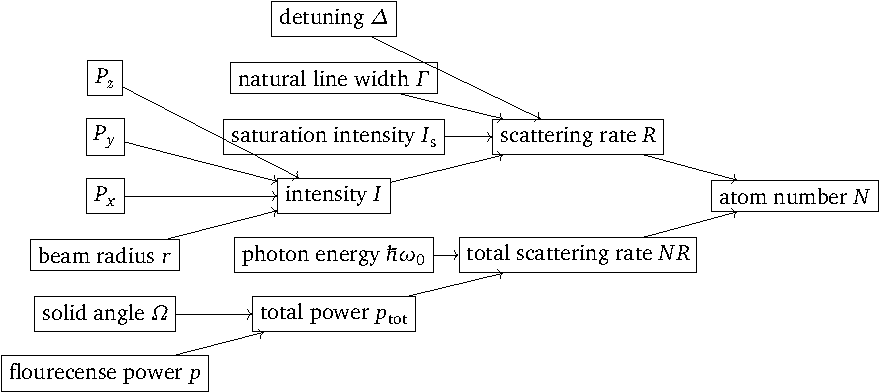
\includegraphics{mot-population-flow}
    \caption{%
        Conversion of quantities to obtain the \mot\ population.
    }
    \label{fig:mot-population-flow}
\end{figure}

We know that the distance between the lens and the \mot\ is $l$. The diameter
of the lens is $d$. Then we can work out the solid angle that is taken up by
the lens. The solid angle is $4 \piup$ for the whole sphere. Therefore we need
to take the ratio of the lens surface ($\piup d^2/4$) and divide it by the total
surface of a sphere at distance $l$, $4 \piup l^2$. In total we will then
obtain
\[
    \Omega = 4 \piup \frac{\piup d^2}{16 \piup l^2} = \frac{\piup d^2}{4 l^2}
    = \SI{<< mot_omega >>}{\steradian} \,.
\]

With that solid angle we can convert the measured power $p = \SI{<<
mot_power_nW >>}{\nano\watt}$ into the actual emitted power of the whole \mot,
$p_\text{tot}$. We do this by dividing through the solid angle:
\[
    p_\text{tot} = p \frac{4 \piup}{\Omega}
    = \SI{<< mot_power_tot_nW >>}{\nano\watt} \,.
\]

With a wavelength of the cooling laser $\lambda$ we can compute the angular
frequency $\omega$ and the photon energy $\hbar\omega$. Dividing the total
power by the energy of a single photon gives us the total scattering rate
\[
    NR = \frac{4 \piup p}{\Omega \hbar \omega} \,.
\]

The beam intensity $I$ is the total energy of the six beams (\SI{<<
total_beam_power_mW >>}{\milli\watt}) divided by the cross sectional area of
the beam, $\pi r^2 = \SI{<< beam_area_cm >>}{\centi\meter\squared}$. We have
\[
    I = 2 \frac{P_x + P_y + P_z}{\pi r^2}
    = \SI{<< intens_mW_cm2 >>}{\milli\watt\per\centi\meter\squared}
    \,,
\]
where the factor two stems from the backreflection of each beam back through
the chamber. With the intensity $I$ we can build up give the scattering rate of
an individual atom:
\[
    R = \frac{(I/I_\mathrm s) \piup \Gamma}{1 + (I/I_\mathrm s) + 4
    (\Delta/\Gamma)^2}
    = \SI{<< scattering_rate_MHz >>}{\mega\hertz}
    \,.
\]
The authors quote the natural line width $\Gamma = \SI{6}{\mega\hertz}$ and
$I_\mathrm s = \SI{4.1}{\milli\watt\per\centi\meter\squared}$.
% TODO Cite (4) from the Wieman paper.
We also need the wavelength $\lambda = \SI{<< wavelength_nm >>}{\nano\meter}$.
Using that we can compute $\hbar\omega = \SI{<< hbar_omega_nW_MHz
>>}{\nano\watt\mega\hertz}$.

Taking all those pieces together we arrive at the expression for the atom
number depending only on observables that we have:
\[
    N = \frac{4 \piup p}{\Omega \hbar \omega} 
    \frac{1 + (I/I_\mathrm s) + 4 (\Delta/\Gamma)^2}{(I/I_\mathrm s) \piup \Gamma}
    = \num{<< atom_number >>}
    \,.
\]

% TODO Obtain the number of atoms in the MOT.

\chapter{Conclusion}

\end{document}

% vim: spell spelllang=en_us tw=79
